\section{Challenged Networks}

Challenged networks are systems that deals with links that have
characteristics very different from the standard ones:

\begin{itemize}
\item satellites links $\to$ they are sensitive to meteorological conditions
  and they have a long RTT
\item 3G, 4G cellular systems
\item WiFi (802.11), WiMax (802.16)
\item fiber Optic Links
\item car-to-car
\item interplanetary net
\end{itemize}

Due to packet losses, dupAcks, timeouts etc\dots the link is never used
to his full potential.

Disruptive/intermitted links: with this kind of links there is no fixed
infrastructure, no antenna and no cable.
In these cases it is not possible to use the usual protocols.
This leads to the following opportunities:
\begin{itemize}
\item ubiquitous computing
\item back-up networks (after-disaster recovery, fast network deployment)
\item always-on connection
\item very fast connection
\item traffic control
\item space communication
\end{itemize}
\dots but with many issues:
\begin{itemize}
\item great increase of RTT
\item there is a PER (Packet Error Rate) not reducible (average: 0-10\%)
\item redundancy is needed
\item the acceleration speed is slow
\end{itemize}
There is an interest in exploiting disruptive links (no end-to-end
connectivity), as for example opportunistic communication.

TCP is not able to distinguish between losses due to errors in links or due
to congestion and it has several timers that would get crazy in case of
intermitted/disruptive links.
Different algorithms are used to address different problems:
\begin{itemize}
\item large RTT
\item high PER
\item high speed
\item disruptive links
\item \dots
\end{itemize}
We'll analyze for every kind of link possible solutions.

\subsection{Satellite communications}
In today's communications there are two types of satellites used:
\begin{itemize}
\item GEO - orbiting at 3600km from earth
\item LEO - orbiting at 100-150km from earth
\end{itemize}
One of the problems of satellite communications is the great RTT\footnote{RTT
  means \textit{Round Trip Time}}. On top of it, there is a non-negligible
Packet Error Rate (influenced by the weather conditions and constellations
positioning), that force the adoption of some CRC\footnote{CRC: cyclic
  redundancy check} system.
To solve these problems, a new protocol needs to be used, and it's TCP Hybla,
covered in~\ref{prt:tcp:hybla}.

\subsection{Terrestrial communications}
Terrestrial communications are:
\begin{itemize}
\item 3-4G
\item WiFi (802.11)
\item WiMAX (802.16)
\end{itemize}

\paragraph*{Characteristics} There are some characteristic in terrestrial
communications: first of all, there is a variable RTT, and, as for satellite
communications there is a non-negligible packet error rate. Finally, there are
performances issues for cabled links (e.g. fiber communications), because
internet protocols aren't able to exploit high-speed networks.

\subsection{TCP solutions}

As we can understand, traditional TCP protocols don't work very well with these
links. High-speed networks requires very high volumes of W\footnote{congestion
window}: $B(t) = \frac{W(t)}{RTT}$, and too little retransmission timers lead
to frequent retransmissions.
Thus, new TCP protocols were made.

\subsubsection{TCP Hybla}
\label{prt:tcp:hybla}

This protocol equalize the transmission rate against the RTT, and it's good for
satellite links.

TCP Hybla adopt the following solution: it sets a new parameter, $\rho$,
setting it to $\rho = \frac{RTT}{RTT_0}$, where $RTT_0$ is a reference RTT
(usually equals to 25ms).
Differently to ``classic'' TCP formula for $W(t)$ that is:
\begin{equation*}
  W(t) = \begin{cases}
    \frac{t}{2 \cdot RTT}, & \mbox{with } 0 \le t < t_y \mbox{ for slow start phase (SS)} \\
    \frac{t - t_y}{RTT} + y, & \mbox{with } t \ge t_y \mbox{ for collision avoidance phase (CA)}
  \end{cases}
\end{equation*}
the Hybla formula for $W(t)$ is:
\begin{equation}
  W(t) = \begin{cases}
    \rho^{2^{\rho \frac{t}{RTT}}} & \mbox{with } 0 \le t < t_{y,0} \mbox{ for slow start phase (SS)} \\
    \rho \cdot \left [\rho\frac{t - t_{y,0}}{RTT} + \gamma \right ] & \mbox{with } t \ge t_{y,0} \mbox{ for collision avoidance phase (CA)}
  \end{cases}
\end{equation}

\paragraph*{Hybla problems} Hybla has some flaws: it's a bit aggressive as
protocol, but its ok cause it'd be too slow otherwise. Keep in mind that being
aggressive means that you risk to lose many packets all together. In this case,
aggressiveness could cause friendliness problems too, such as disruption of
other protocols.
When the RTT is big it'll cause even more aggressiveness, and the solution to
this is to provide bigger buffers, that's bad for real time communications.

\subsubsection{TCP High-speed}
The aim of this protocol is to improve the exploitation of high-speed network
bandwidth (e.g. fiber links). Similar to Hybla, when the cwnd is high, it's
more aggressive.

\subsubsection{Disruption Tolerant Networks - DTN}
DTN are designed to work whenever end-to-end connectivity may be not always
available. DTN adds a new layer (bundle layer) under the application one, that
sends the messages to the network as soon as it's available, creating a TCP
connection.
\begin{itemize}
\item Pro:
  \begin{itemize}
  \item no end-to-end TCP semantics violation
  \end{itemize}
\item Cons:
  \begin{itemize}
  \item the new bundle creates a little overhead
  \end{itemize}
\end{itemize}

\begin{figure}[H]
  \centering
  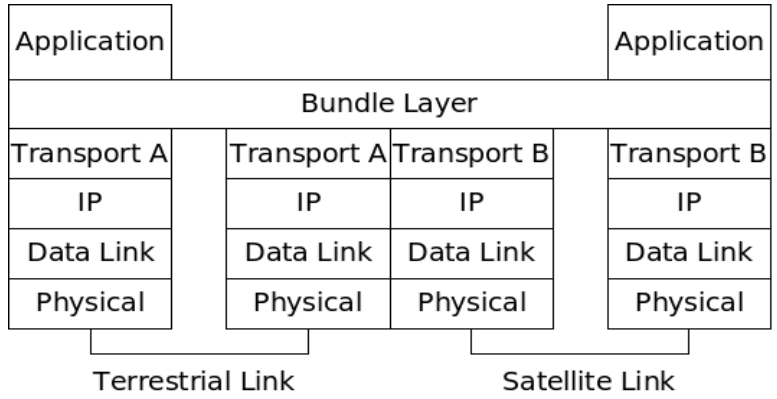
\includegraphics[scale=0.45]{DTNStack}
  \caption{DTN Stack}
\end{figure}

\subsubsection{Performance Enhancing Proxies}
This proxy isolates the challenge link with the rest of the network, through an
intermediate agent before it.
\begin{itemize}
\item Pro:
  \begin{itemize}
  \item performance boost
  \item can support every TCP enhancement
  \end{itemize}
\item Cons:
  \begin{itemize}
  \item violation of the TCP end-to-end semantics
  \item no IPSec support
  \end{itemize}
\end{itemize}

\subsubsection{TCP adaptive - Selection}
Proposed from the DTN group, the right TCP protocol is selected based on the
connection. This selection is performed using the following characteristics:
\begin{itemize}
\item from the agent that perform TCP selection
\item exploiting cross-layer possibilities
\item changing TCP protocol on-the-fly, even if it's not easy
\end{itemize}

\subsection{Summary}
None of this solutions solve all the problems. At the end, the server always
needs to change the TCP implementation.
